\beginsong{Raubritter}[
    wuw={nathan (Georg Hausmann) und anti (Volker Hausmann), Nerother Wandervogel}, 
    jahr={1967}, 
    bo={344}, 
    pfii={16}, 
    pfiii={6}, 
    gruen={153}, 
    kssiv={33}, 
    siru={241}, 
    index={Von der Festung dröhnt},
]

\beginverse
\endverse
\centering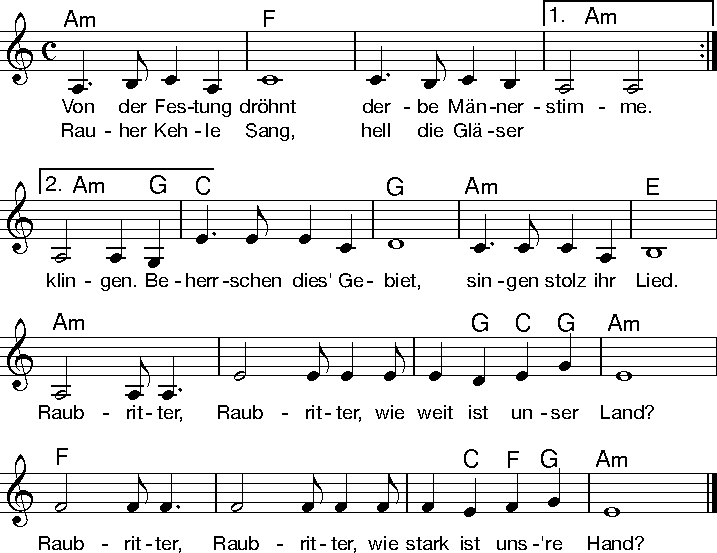
\includegraphics[width=1\textwidth]{Noten/Lied077.pdf}	 

\beginverse
\[Am]In uns'rer Knechtschaft \[F]Zeit griffen wir zu \[Am]Waffen,
schlugen uns're \[F]Herr'n, Grafen und auch \[Am]Pfaffen.
\endverse

\beginchorus
\[G]Be\[C]herrschen dies Ge\[G]biet, \[Am]singen stolz ihr \[E]Lied: 
\[Am]Raubritter, Raubritter, wie weit \[G]ist \[C]un\[G]ser \[Am]Land?
\[F]Raubritter, Raubritter, wie stark \[C]ist \[F]uns'\[G]re \[Am]Hand?
\endchorus
 
\beginverse
^Groß ist uns're ^Macht, solange wir ^vereint.
Hüten uns're ^Burg, trotzen jedem ^Feind.
\endverse

\renewcommand{\everychorus}{\textnote{\bf Refrain (wdh.)}}
\beginchorus
\endchorus

\endsong

\beginscripture{}
Im Jahre 1967 spaltete sich der Orden der Raubritter vom Orden der Rabenklaue im Nerother Wandervogel ab. Das Lied wurde das Ordenslied des neu gegründeten Ordens. Es existieren viele Textvariationen, die vermutlich durch die mündliche Übetragung entstanden sind.

Als Raubritter bezeichnet man diejenigen Angehörigen des ritterlichen Standes, die sich durch Straßenraub, Fehden und Plünderungszüge bereicherten.
\endscripture
